\documentclass[11pt]{article}
\usepackage{geometry} % Pour passer au format A4
\geometry{hmargin=0.8cm, vmargin=0.8cm} % 

% Page et encodage
\usepackage[T1]{fontenc} % Use 8-bit encoding that has 256 glyphs
\usepackage[english,french]{babel} % Français et anglais
\usepackage[utf8]{inputenc} 

\usepackage{lmodern}
\setlength\parindent{0pt}

% Graphiques
\usepackage{graphicx,float,grffile}

% Maths et divers
\usepackage{amsmath,amsfonts,amssymb,amsthm,verbatim}
\usepackage{multicol,enumitem,url,eurosym,gensymb,multido,enumitem}

% Sections
\usepackage{sectsty} % Allows customizing section commands
\allsectionsfont{\centering \normalfont\scshape}

% Tête et pied de page

\usepackage{fancyhdr} 
\pagestyle{fancyplain} 

\fancyhead{} % No page header
\fancyfoot{}

\renewcommand{\headrulewidth}{0pt} % Remove header underlines
\renewcommand{\footrulewidth}{0pt} % Remove footer underlines

\newcommand{\horrule}[1]{\rule{\linewidth}{#1}} % Create horizontal rule command with 1 argument of height

\newcommand{\Pointilles}[1][3]{%
  \multido{}{#1}{\makebox[\linewidth]{\dotfill}\\[\parskip]
}}

\setlength{\columnseprule}{1pt}
\renewcommand{\labelitemii}{$\star$}
\renewcommand{\labelitemi}{$\bullet$}

\begin{document}

\textbf{Nom, Prénom :} \hspace{8cm} \textbf{Classe :} \hspace{3cm} \textbf{Date :}\\

\begin{center}
  \textit{Observer attentivement, c'est se rappeler distinctement.}  - \textbf{Edgar Allan Poe}
\end{center}


\subsection*{ex1 : Réduire}

\textit{Réduire les expressions quand cela est possible.}

\begin{multicols}{3}

\begin{itemize}
  \item[$\bullet$] $2x + x = \dotfill$ 
  \item[$\bullet$] $3 \times x + 1 = \dotfill$
  \item[$\bullet$] $5 \times x \times 2 = \dotfill$ 
  \item[$\bullet$] $6x + 4 + 4 x= \dotfill$
  \item[$\bullet$] $1 + 2 \times x + 9 = \dotfill$
  \item[$\bullet$] $5x - 4 \times x = \dotfill$
  \item[$\bullet$] $x - x = \dotfill$
  \item[$\bullet$] $-4x + -12x = \dotfill$
  \item[$\bullet$] $2 \times x \times x \times 5 = \dotfill$
  \item[$\bullet$] $0 \times x + 4 + 5x = \dotfill$
  \item[$\bullet$] $2a + 2b + 6a + 4 = \dotfill$
  \item[$\bullet$] $-x + -10x + 6 = \dotfill$ 
\end{itemize}

\end{multicols}

\subsection*{ex2 : Calculer}

\textit{Écrire le calcul et la réponse.}

\begin{multicols}{2}
\textit{On pose :$a = 12$ et $b = 5$. }

\begin{itemize}
  \item[$\bullet$] $2a + 3b + 2 = \dotfill$
  \item[$\bullet$] $a \times (b - 2) = \dotfill$
  \item[$\bullet$] $10 \times a \times b - 10b = \dotfill$
  \item[$\bullet$] $\dfrac{a}{b + 1} + b = \dotfill$
  \item[$\bullet$] $(a + b) \times (a - b) = \dotfill$
\end{itemize}

\columnbreak

\textit{On pose : $a = 5$ et $b = -4$.}

\begin{itemize}
  \item[$\bullet$] $2a + 3b + 2 = \dotfill$
  \item[$\bullet$] $a \times (b - 2) = \dotfill$
  \item[$\bullet$] $10 \times a \times b - 10b = \dotfill$
  \item[$\bullet$] $\dfrac{a}{b + 1} + b = \dotfill$
  \item[$\bullet$] $(a + b) \times (a - b) = \dotfill$     
\end{itemize}
\end{multicols}
\subsection*{ex3 : Modéliser un problème}
\textit{Sans chercher à résoudre le problème, modéliser les problèmes suivants.}

\begin{multicols}{2}
\begin{enumerate}
  \item[1.] Manu a obtenu 11, 14 et 16 aux trois premiers contrôles de Maths. Quelle note doit-il avoir au quatrième contrôle pour obtenir 15 de moyenne ?
  \item[2.] Gégé a le double de l’âge de sa fille. Dans 10 ans il aura le triple de son âge actuelle. Quel est l’âge de la fille ?
  \item[3.] Jean Mi a achète 22 ballons de foot, 10 ballons de basket et 10 ballons de rugby. Un ballon de basket coûte 2 € de plus qu’un ballon de foot. Une ballon de rugby coûte 2 fois plus cher qu'un ballon de foot.  Il dépense en tout 540 €. Quel est le prix de chaque sorte de ballon ?
\end{enumerate}
\columnbreak
\Pointilles[24] 
\end{multicols}
\newpage

\begin{multicols}{2}
  \subsection*{ex4 : Modéliser un graphique}
  \begin{enumerate}
  \item[1.] Représenter les figures manquantes.
  \item[2.] Calculer les aires de chacune des figures.
  \item[3.] Calculer l'aire pour $n = 10$. (écrire le calcul ou la démarche)
  \item[4.] Modéliser une formule pour $n = x$
\end{enumerate}
\end{multicols}

\begin{figure}[H]
      \centering
      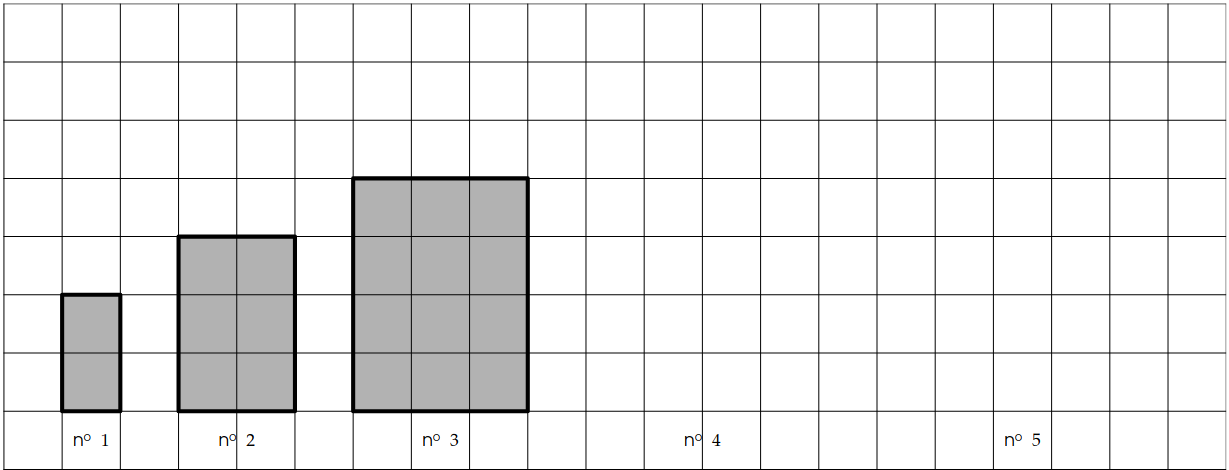
\includegraphics[width=0.7\linewidth]{5x11-calcul-litteral/sources/geo-1.png}
\end{figure}

\Pointilles[4]

\begin{figure}[H]
      \centering
      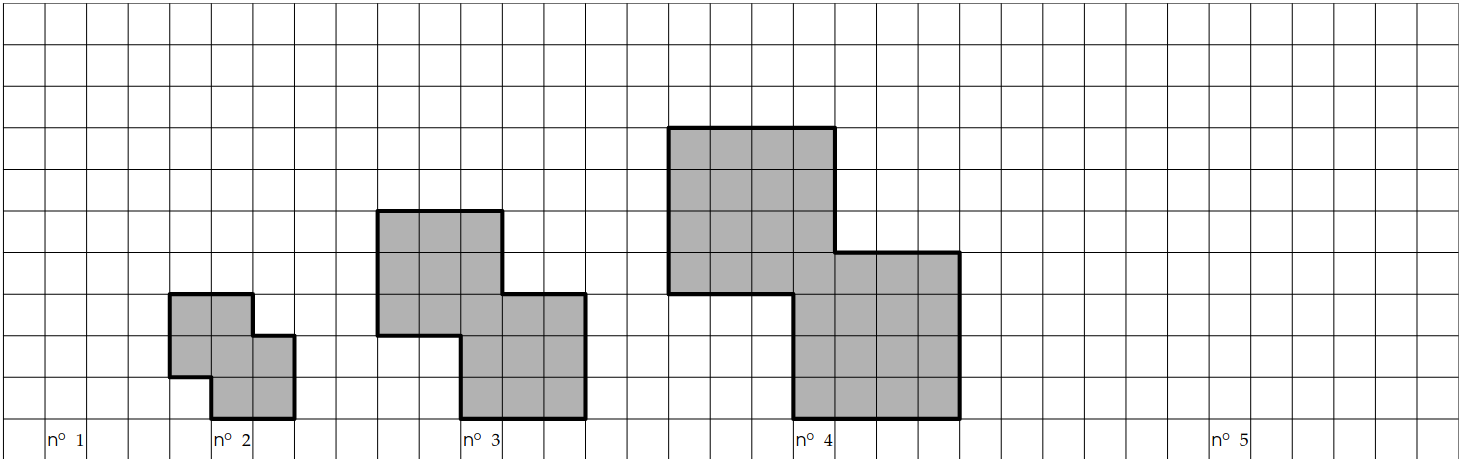
\includegraphics[width=0.7\linewidth]{5x11-calcul-litteral/sources/geo-2.png}
\end{figure}

\Pointilles[4]

\begin{figure}[H]
      \centering
      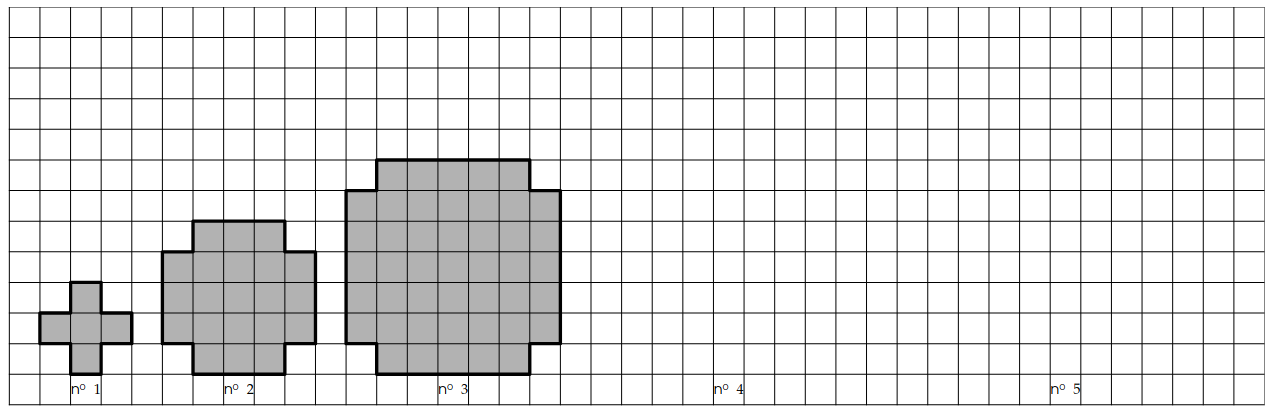
\includegraphics[width=0.7\linewidth]{5x11-calcul-litteral/sources/geo-3.png}
\end{figure}

\Pointilles[4]

\end{document}